\documentclass[11pt]{amsart}

% Standard letter size paper with 1inch margins
\usepackage[letterpaper, margin=1in]{geometry}
\usepackage{float}
% Useful packages 
\usepackage{amsmath, amssymb, amsthm, amsaddr}
\usepackage{enumerate, subcaption, graphicx, hyperref}
\usepackage{xcolor}
\usepackage{diagbox}
\raggedbottom



\title{AMATH 482/582: Homework 5}
\author{Sathvik Chinta} % first and last name

\date{\today} % you can also just type the date instead of "\today"

\begin{document}

\maketitle 

\begin{abstract}
    Using the discrete cosine transform and solving optimization problems, we are 
    able to reconstruct corrupter (and mysterious) images to a very high degree of 
    clarity. 
    % Your report should contain a brief, 100 word abstract describing what is contained in 
    % the document and what you did. {\bf Don't forget 6 pages max}.
\end{abstract}


\section{Introduction and Overview}\label{sec:Introduction}
Imagine we are given an image that is corrupted. Can we reconstruct said image using what we have learned so far? 
In our effort to do so, we will go back to Fourier Transforms and apply them to the image.
However, instead of regular Fourier transforms, we will instead be using the Discrete Cosine Transform.

We will first identify the compressibility of the image using the DCT. 
Then, we will attempt to recover the corrupted image using the inverse DCT. Finally, we 
will apply all methods to find out what the mystery image we are given is. 
% You dedicate this section to the theoretical background of the methods and frameworks 
% that you used in your homework. This is not meant to reproduce material from the lectures
%  or references you used but rather to demonstrate your understanding of the 
%  mathematical foundations of the methods and algorithms. You can create equations like this 
%  \begin{equation*}
%      f(x) = \int_A \sin( \pi x) dx.
%  \end{equation*}
%  You do not need to label your equations unless they are referenced in the text. In that 
%  case simply use 
%  \begin{equation}\label{eq:meaningful-label}
%       - \frac{\partial^2 u}{\partial x^2} = \sin ( \pi x).
%  \end{equation}
% Also look up the \texttt{align} or \texttt{aligned} environments if you want multi-line 
% equations. You can then reference your equations in text using the $\backslash$\texttt{eqref}
% command as such \eqref{eq:meaningful-label}. 

\section{Theoretical Background}\label{sec:theory}

We will first take the discrete cosine transform of our image. 
The discrete cosine transform is a fast way to compute the Fourier transform of a discrete signal.
The discrete cosine transform is very similar to the discrete Fourier transform, but we 
only use real numbers. 

So, where DFT will use both sine and cosine waves, the discrete 
cosine transform only breaks the signal up into cosine waves. We can define 
the DCT of a real signal $f \in \mathbb{R}^K$ as 

\[DCT(f)_k = \sqrt{\frac{1}{K}}[f_o\cos(\frac{\pi k}{2K}) + \sqrt{2}\sum_{j = 1}^{k-1}{f_j\cos(\frac{\pi k(2j + 1)}{2K})}]\]

Let's take our SonOfMan image and then investigat the compressibility of its 
Discrete Cosine Transform. This just involves us passing the pixel values (flattened) 
into the equation above. We can then investigate the size of the coefficients. If there are 
not many large coefficients, then the image is very compressible. 

Once we do that, we can reconstruct the image after keeping a certain amount of 
the coefficeints, and we can extrapolate what we learn to figure out if we can recover the original image or not. 

From the original image, we can then attempt to solve the optimization problem 

\[\text{minimize}_{x \in \mathbb{R}^N} ||x||_1\]
\[\text{Subject to } Ax = y\]

Where $x$ is the DCT vector of our corrupted image, $y$ is 
our vector of measurements, and $A$ is constructed using a combination 
of our inverse DCT and random rows of the identity matrix (of dimension $N$ where $N$ is the 
number of pixels in our image).



\section{Algorithm Implementation and Development}\label{sec:algorithms}
I used Python in conjunction with NumPy, Matplotlib, cvxpy, and scipy

I first used the scipy.spfft.dct() function to compute the DCT matrix,
and then used the scipy.spfft.idct() to compute the inverse DCT matrix. Then I took 
the dot product between my image (flattened) and the DCT matrix to get the DCT coefficients
(stored as $DCT_F$).

After looking at the DCT coefficients, I used the np.percentile() function to get the 
threshold value for each percentage within the array [5, 10, 20, 40]. Then I looped through 
my $DCT_F$ value and set all values (absolute) below the threshold to 0. Once this 
was done, I applied the inverse DCT to the resulting array to get the 
image with only a certain percentage of the coefficients. 

To reconstruct the corrupt image, I first used the np.random.percentile() function on the 
identity matrix (with dimensionality equivalent to my image size), and took the first M rows 
(percentage of my image size) to compute my $M$ matrix. I then found the $y$ value by 
multiplying my my flattened image, and my $A$ matrix by multiplying the $B$ matrix by 
the inverse DCT matrix. I then used the CVXPY library with the CVXOPT solver to solve 
the optimization problem of minimizing the one-norm of x subject to $Ax = y$. Then I took 
the dot product between this value ($x^*$) and multiplied it by the inverse DCT matrix 
to get my final image. I did this three times for each percentage within r = [0.2, 0.4, 0.6] to get a diverse subset of 
the random B matrix, and plotted the results. 

Finally, I used a simlar form of solving to extract the mystery image. The $B$ and $y$ matrices
were already provided, so I just had to plug them into the same CVXOPT solver to reconstruc the final image. 


% Here you discuss the algorithms and software packages that you used. Not much to it. 
% Just make sure you cite the packages properly and avoid including code. 
% You are welcome to use \LaTeX packages that are specifically designed to show 
% algorithms such \href{https://www.overleaf.com/learn/latex/Algorithms}{as this}, but it is 
% not always worth the effort and real estate. 


\section{Computational Results}\label{sec:results}

After calculating the DCT matrix and applying it to our image, I 
got the following result for the coefficeints. 

\begin{figure}[H]
    \centering
    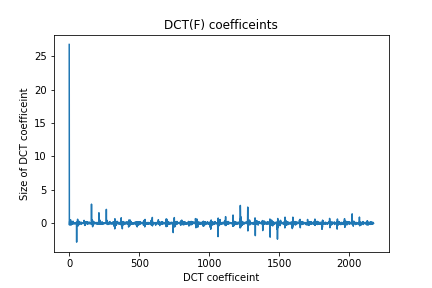
\includegraphics[width=0.91\textwidth]{/home/sathvikc/AMATH-482-2/AMATH-482/Homework Assignments/Homework 5/DCT_F_coefficients.png}
    \caption{DCT Coefficients of SonOfMan image}
    \label{fig:DCTCoef}
\end{figure}

We can see that the coefficients start out very large, then quickly become 
quite relatively small. After about 1500 coefficients, the absolute value 
of the coefficeints becomes even smaller. This indicates that the image is very compressible 

Looking at the image with only a percentage of the coefficients we get the following result: 

\begin{figure}[H]
    \centering
    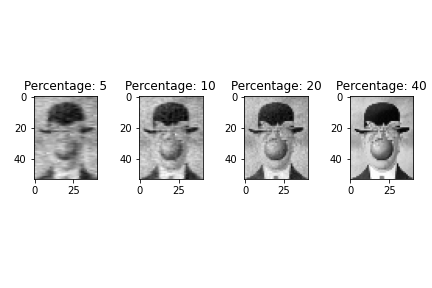
\includegraphics[width=0.8\textwidth]{/home/sathvikc/AMATH-482-2/AMATH-482/Homework Assignments/Homework 5/DCT_F_coefficients_cutoff.png}
    \caption{First DCT Coefficients of SonOfMan image broken up by percentages}
    \label{fig:DCTCoefPercentage}
\end{figure}

We can see that keeping only 5\% of the image 
does not result in a clear image, but at 40\% we get a very clear image! In fact, 
we can see a surprising amount of detail at 20\%, and a case could be made for using just 10\% of the 
coefficients! This image is very compressible, just as we predicted. 

Using our optimizer to recover the image, we get the following results:

\begin{figure}[H]
    \centering
    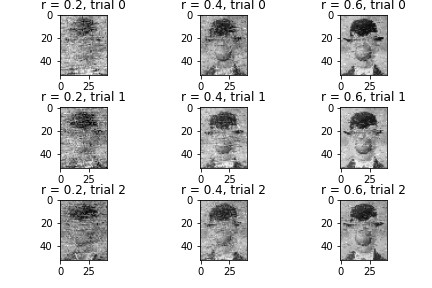
\includegraphics[width=0.65\textwidth]{/home/sathvikc/AMATH-482-2/AMATH-482/Homework Assignments/Homework 5/F_recovery.png}
    \caption{Reconstructing the SonOfMan image using the DCT with varying matrix sizes}
    \label{fig:Reconstructed Image}
\end{figure}

We can see that we are able to recover the original image very well! When r = 0.6, 
we naturally have the most clarity. However, across multiple trials, we can also see that 
r = 0.4 provides good results as well. It makes sense that we need a larger percentage to 
reconstruct an image if the image was originally corrupted, but we can surprisingly see 
a lot more detail in the image than was present in the corrupted version!

Finally, let's see if we can apply the same 
methodology on an unknown mystery image. Performing the same optimization problem 
here, we get 

\begin{figure}[H]
    \centering
    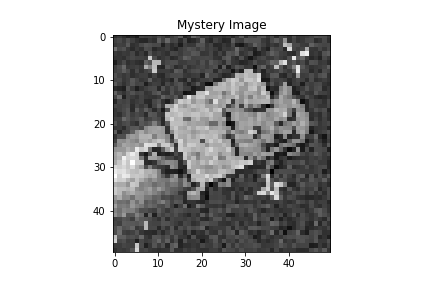
\includegraphics[width=1\textwidth]{/home/sathvikc/AMATH-482-2/AMATH-482/Homework Assignments/Homework 5/MysteryImage.png}
    \caption{A Mysterious Image Reconstructed!}
    \label{fig:Nyan_Image}
\end{figure}

It works! We're able to reconstruct the mystery image 
to a remarkable degree of clarity. We can see that this image is none other than Nyan Cat! 
%This is perhaps the most important section of your report. You want to dedicate more space 
% here and present your numerical results in a clear, concise and meaningful way. Also 
% include a discussion of your numerics. Think hard about how you can use 
% your space most efficiently. For example, include subplots and multiple error curves on the 
% same plot etc. Ask us for advice when the time comes. 

% You will most definitely need tables and figures. So here is an example. 

% \begin{table}[htp]
%     \centering
%     \begin{tabular}{| l | c|c | r |}
%          \hline
%          row 1 & column 1  & column 2  \\ \hline
%          row 2 & column 1 & column 2 \\ 
%          row 3 & column 1 & column 2 \\ \hline
%     \end{tabular}
%     \caption{Don't forget to include a caption for your table. Say a few words about what is 
%     being shown.}
%     \label{tab:meaningful-label}
% \end{table}

% Make sure your table is labeled and referenced withing the text using $\backslash$\texttt{ref} as such Table~\ref{tab:meaningful-label}. In fact, you can 
% use $\backslash$\texttt{ref} to cite anything else in the document such as 
% sections (ex. Section~\ref{sec:Introduction}). This will create hyperlinks in your 
% pdf after compilation and automatically update the numbers and tags whenever you change 
% anything. 

% Figures are very similar to tables. Here's an example: 

% % \begin{figure}[htp]
% %     \centering
% %     \includegraphics[width=0.4\textwidth]{./Figs/fig1.pdf}
% %     \caption{Include a descriptive caption for your figure. Also make sure all 
% %     legends, axis labels, and titles are large enough to be readable. You might have 
% %     to reproduce the plots from Python or MATLAB with larger fonts for this purpose. It 
% %     can be annoying the first time you do it but it is crucial.}
% %     \label{fig:meaningful-label}
% % \end{figure}

% You may also need to include multiple figures: 

% % \begin{figure}
% %     \centering
% %     \begin{subfigure}[b]{.3\textwidth}
% %     \includegraphics[width=\textwidth]{./Figs/fig1.pdf}
% %     \caption{First subfigure}
% %     \label{subfig:first}
% %     \end{subfigure}
% %     \begin{subfigure}[b]{.3\textwidth}
% %     \includegraphics[width=\textwidth]{./Figs/fig2.pdf}
% %     \caption{First subfigure}
% %     \label{subfig:second}
% %     \end{subfigure}
% %     \begin{subfigure}[b]{.3\textwidth}
% %     \includegraphics[width=\textwidth]{./Figs/fig3.pdf}
% %     \caption{First subfigure}
% %     \label{subfig:third}
% %     \end{subfigure}
% %     \caption{Caption for entire figure. You don't need to use captions for subfigs so 
% %     feel free to eliminate the subcaption texts to just have the A, B, C labels.}
% %     \label{fig:meaningful-label-2}
% % \end{figure}

% Once again, make sure all your figures are referenced like Figure~\ref{fig:meaningful-label}
% or Figure~\ref{subfig:first} in the text body of the report and discussed 
% in detail. This is where you will make observations about your results and we will 
% look at these very closely. 

% Also note, I am using PDF figures. These give you the best looking graphs but PNG works 
% well too. I advise staying away from JPG as it always looks weird and low quality.]
% Both Python and MATLAB can output figures in PDF or PNG.

\section{Summary and Conclusions}\label{sec:conclusions}
We have seen that using our already pre-existing knowledge, we can re-construct 
images to a very high degree of clarity. We have also seen that we can use our
knowledge to construct corrupted images even when we don't know the compressibility of it, as 
shown by Nyan Cat. 

% Wrap up your report with a brief summary of what you did and what you discovered. 
% Finish with some conclusions and possibly future directions if any. 

\section*{Acknowledgements}
I am thankful to Professor Hosseini for introducing us to the concept of Fourier transforms, and by extension
allowing us to learn about Discrete Fourier Transforms. Furthermore, I would also like to thank 
Professor Hosseini for 

I am very thankful to my peers taking the class alongside me, they have helped me understand the material as well
as provide a reference to compare my results against. I interacted with them both through Canvas discussion boards
as well as Discord chat. 
% Make sure you you clearly state any help you received including collaborations 
% with your peers. Help from TAs or other mentors, professors, etc that helped you 
% with your assignment. Here's a formal example: 

% The author is thankful to Prof. X for useful discussions about the QR algorithm. 
% We are also thankful to Dr. Strange for suggesting the JAX software package for 
% automatic differentiation. Furthermore, our peer Jean Grey was helpful in 
% implementation of spectral clustering in Python.

 % make sure this matches the .bib file for your corresponding document. You also have to maintain your references in the .bib file 

\bibliographystyle{abbrv}
\bibliography{HW_References}
\cite{Hunter:2007}
\cite{harris2020array}
\cite{scikit-learn}
\cite{diamond2016cvxpy}

\end{document}
